\documentclass[]{article}
\usepackage{lmodern}
\usepackage{amssymb,amsmath}
\usepackage{ifxetex,ifluatex}
\usepackage{fixltx2e} % provides \textsubscript
\ifnum 0\ifxetex 1\fi\ifluatex 1\fi=0 % if pdftex
  \usepackage[T1]{fontenc}
  \usepackage[utf8]{inputenc}
\else % if luatex or xelatex
  \ifxetex
    \usepackage{mathspec}
  \else
    \usepackage{fontspec}
  \fi
  \defaultfontfeatures{Ligatures=TeX,Scale=MatchLowercase}
\fi
% use upquote if available, for straight quotes in verbatim environments
\IfFileExists{upquote.sty}{\usepackage{upquote}}{}
% use microtype if available
\IfFileExists{microtype.sty}{%
\usepackage{microtype}
\UseMicrotypeSet[protrusion]{basicmath} % disable protrusion for tt fonts
}{}
\usepackage[margin=1in]{geometry}
\usepackage{hyperref}
\hypersetup{unicode=true,
            pdftitle={Data Science for Industry Project 2},
            pdfborder={0 0 0},
            breaklinks=true}
\urlstyle{same}  % don't use monospace font for urls
\usepackage{graphicx,grffile}
\makeatletter
\def\maxwidth{\ifdim\Gin@nat@width>\linewidth\linewidth\else\Gin@nat@width\fi}
\def\maxheight{\ifdim\Gin@nat@height>\textheight\textheight\else\Gin@nat@height\fi}
\makeatother
% Scale images if necessary, so that they will not overflow the page
% margins by default, and it is still possible to overwrite the defaults
% using explicit options in \includegraphics[width, height, ...]{}
\setkeys{Gin}{width=\maxwidth,height=\maxheight,keepaspectratio}
\IfFileExists{parskip.sty}{%
\usepackage{parskip}
}{% else
\setlength{\parindent}{0pt}
\setlength{\parskip}{6pt plus 2pt minus 1pt}
}
\setlength{\emergencystretch}{3em}  % prevent overfull lines
\providecommand{\tightlist}{%
  \setlength{\itemsep}{0pt}\setlength{\parskip}{0pt}}
\setcounter{secnumdepth}{0}
% Redefines (sub)paragraphs to behave more like sections
\ifx\paragraph\undefined\else
\let\oldparagraph\paragraph
\renewcommand{\paragraph}[1]{\oldparagraph{#1}\mbox{}}
\fi
\ifx\subparagraph\undefined\else
\let\oldsubparagraph\subparagraph
\renewcommand{\subparagraph}[1]{\oldsubparagraph{#1}\mbox{}}
\fi

%%% Use protect on footnotes to avoid problems with footnotes in titles
\let\rmarkdownfootnote\footnote%
\def\footnote{\protect\rmarkdownfootnote}

%%% Change title format to be more compact
\usepackage{titling}

% Create subtitle command for use in maketitle
\newcommand{\subtitle}[1]{
  \posttitle{
    \begin{center}\large#1\end{center}
    }
}

\setlength{\droptitle}{-2em}
  \title{Data Science for Industry Project 2}
  \pretitle{\vspace{\droptitle}\centering\huge}
  \posttitle{\par}
  \author{}
  \preauthor{}\postauthor{}
  \date{}
  \predate{}\postdate{}

\usepackage{graphicx}
\usepackage{float}
\usepackage{booktabs}
\usepackage{longtable}
\usepackage{array}
\usepackage{multirow}
\usepackage[table]{xcolor}
\usepackage{wrapfig}
\usepackage{float}
\usepackage{colortbl}
\usepackage{pdflscape}
\usepackage{tabu}
\usepackage{threeparttable}
\usepackage{threeparttablex}
\usepackage[normalem]{ulem}
\usepackage{makecell}
\usepackage[english]{babel}
\usepackage[utf8]{inputenc}
\usepackage{algorithm}
\usepackage[noend]{algpseudocode}

\begin{document}
\maketitle

\section{Introduction}

\section{Exploratory Data Analysis}

The data set consists of 30 State of the Nation Address (SONA) speech
transcripts from all the presidents from February 1994 til recently in
February 2018.

A hypothesis can be made that sentiments of speeches differ depending on
the political season.There are 3 political seasons :

\begin{enumerate}
\item Pre-Election
\item Post-Election
\item Normal Term
\end{enumerate}

Below is a summary of all the speeches as per the various presidents
categorized by the 3 political seasons :

\begin{table}[h]
\centering
\begin{tabular}{|l|l|c|c|c|c|}
\hline
\multicolumn{1}{|c|}{Period} & Presidents & \multicolumn{1}{l|}{Pre-Election} & Post-Election & \multicolumn{1}{l|}{Normal Term} & \multicolumn{1}{l|}{\textbf{Total}} \\ \hline
1994                         & de-Klerk   & 1                                 &               &                                  & \textbf{1}                          \\ \hline
1994-1999                    & Mandela    & 1                                 & 2             & 4                                & \textbf{7}                          \\ \hline
2000-2008                    & Mbeki      & 1                                 & 1             & 8                                & \textbf{10}                         \\ \hline
2009                         & Motlante   & 1                                 &               &                                  & \textbf{1}                          \\ \hline
2009-2017                    & Zuma       & 1                                 & 2             & 7                                & \textbf{10}                         \\ \hline
2018                         & Ramaphosa  &                                   &               & 1                                & \textbf{1}                          \\ \hline
\textbf{Total}               &            & \textbf{5}                        & \textbf{5}    & \textbf{20}                      & \textbf{30}                         \\ \hline
\end{tabular}
\caption{The number of SONA per president and arranged by political seasons}
\label{my-label}
\end{table}

From the table above the following remarks can be made :

\begin{itemize}
\item de Klerk,Motlante and Ramaphosa all have one speech each which will make it extremely difficult to accurately predict given the far higher number of speeches from their counterpart presidents.
\item There are far more speeches done during the normal season which will inherently bias the training data towards that season
\item Mbeki and Mandela dominate the number of speeches with 10 apiece.This will also inherently bias the training data towards them.
\item Pre-Election speeches are evenly distributed across 5 of the 6 presidents whilst post election speeches are dominated by Mandela and Zuma.
\end{itemize}

\newpage

\subsection{Word Distribution}

Below are the most frequently used words of all the 30 presidential
speeches rescaled according to their respective political seasons :

\begin{figure}[H]

{\centering 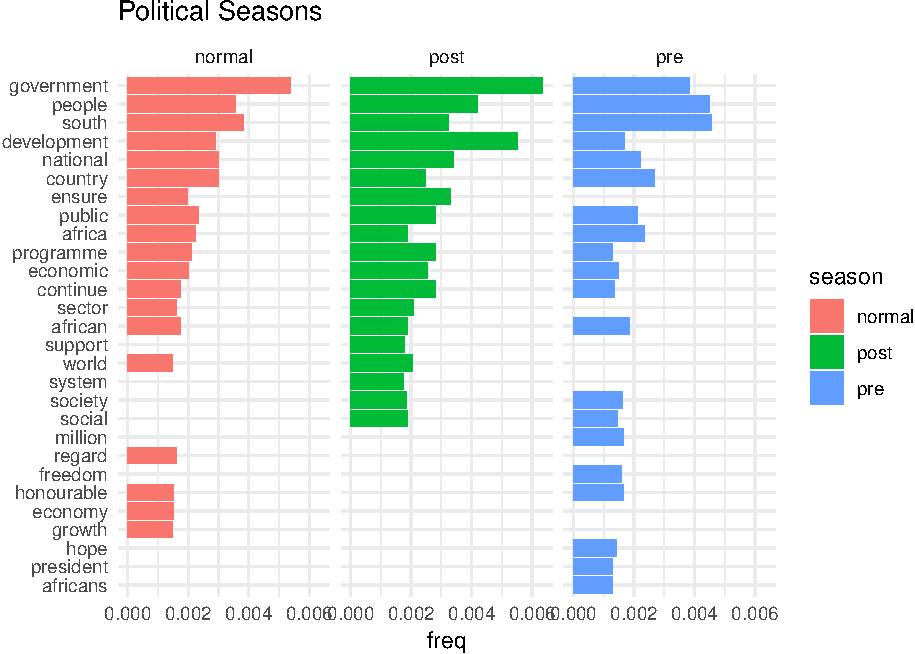
\includegraphics{datasci_fi_Assignment_2_files/figure-latex/eda_season -1} 

}

\caption{Frequently used words across political seasons}\label{fig:eda_season }
\end{figure}

From the illustration above the following remarks can be made :

\begin{itemize}
\item Notable words commonly used across all political seasons are \textbf{south}, \textbf{africa},\textbf{government},\textbf{development},\textbf{people},\textbf{country},\textbf{programme}.These words will potentially not assist in distinguishing the respective presidents.

\item Comparing pre and post to normal political seasons ,notable words like \textbf{economy} and \textbf{growth} are introduced into their speeches .The utilization of these words (which could imply economic growth) are understandable given that these are typical themes that need to be addressed constantly throughout the normal period of presidential terms.

\item Comparing pre to post political seasons,uplifting words like \textbf{freedom},\textbf{hope},\textbf{africans} are used before and not after elections.

\item Comparing pre to post political seasons,notable words introduced are \textbf{support},\textbf{system},\textbf{ensure}.These words convey a theme of action and execution which is expected after coming from an election.

\end{itemize}

Below are the most frequently used words of all the 30 presidential
speeches rescaled according to the respective presidents :

\begin{figure}[H]

{\centering 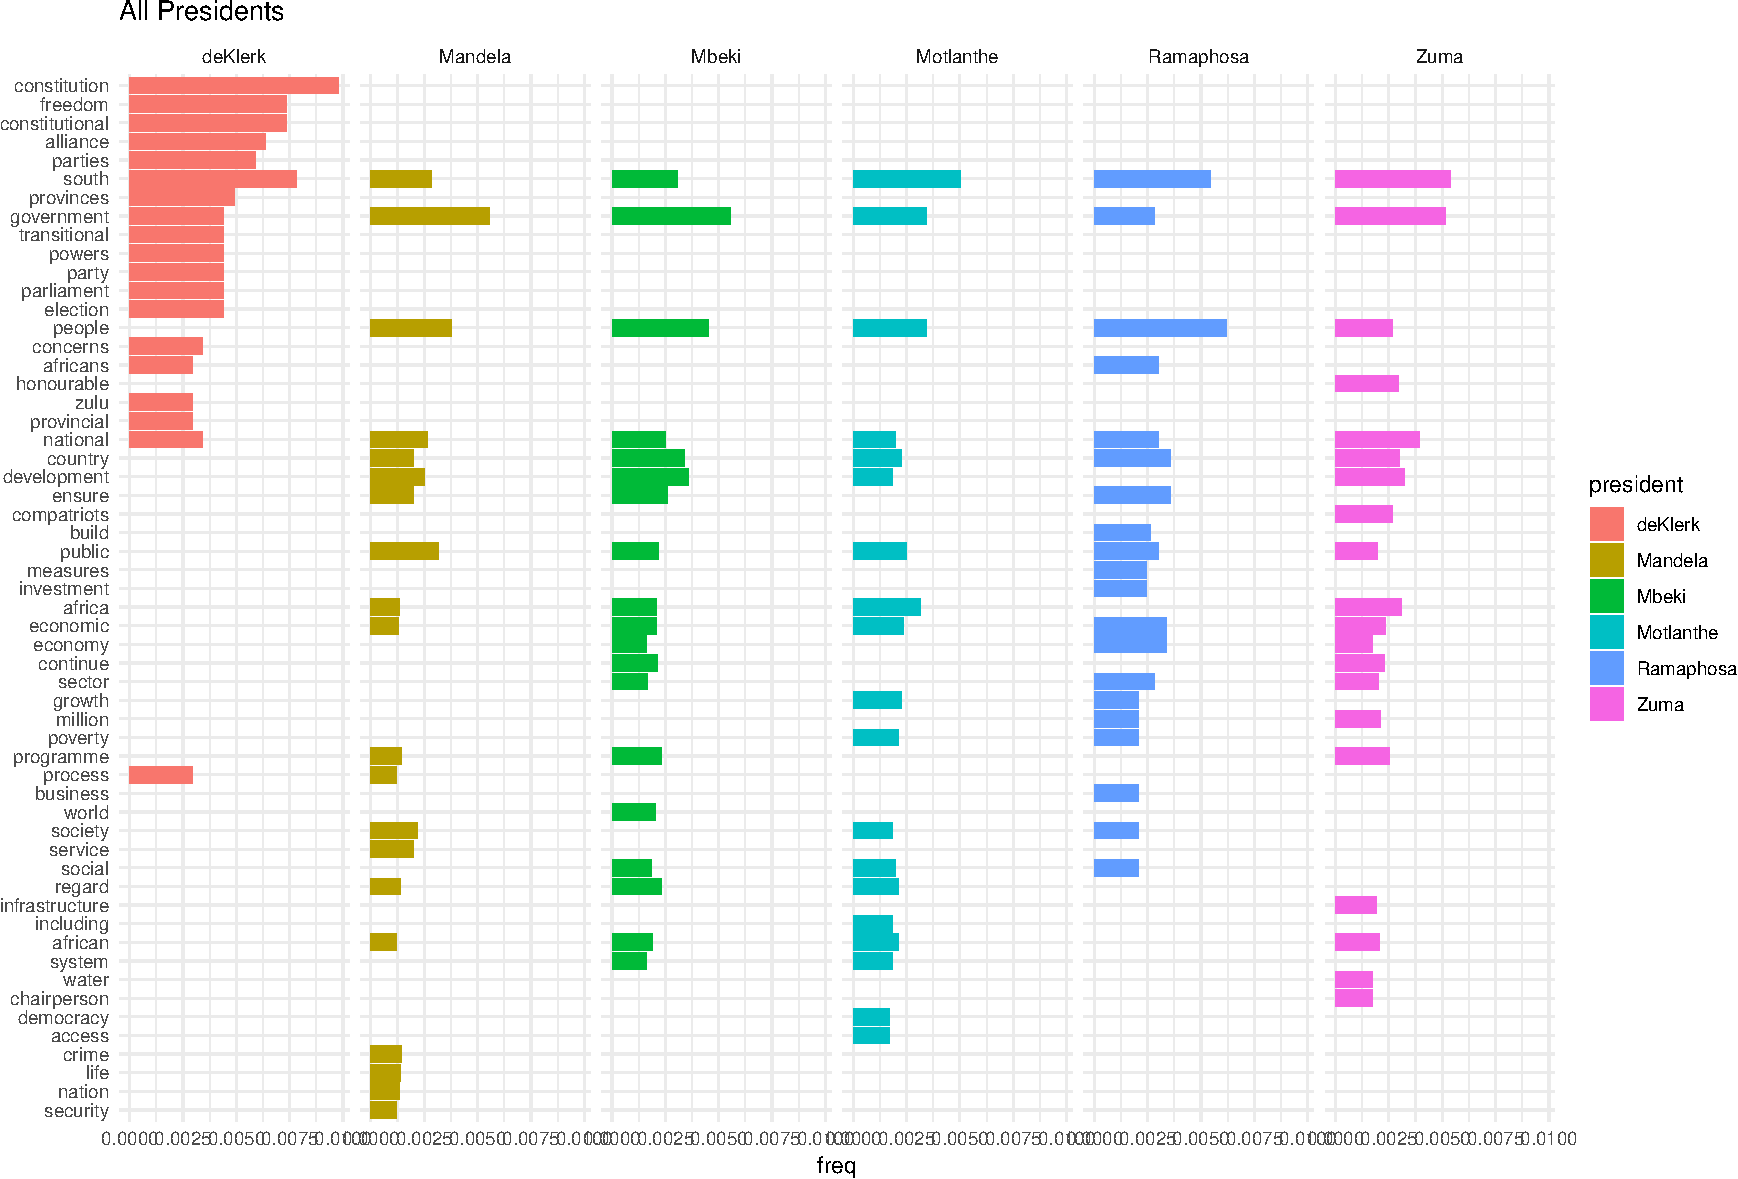
\includegraphics{datasci_fi_Assignment_2_files/figure-latex/eda_presi -1} 

}

\caption{Top words used by all presidents in SONA}\label{fig:eda_presi }
\end{figure}

From the illustration above the following remarks can be made :

\begin{itemize}
\item Looking at all the presidents frequently used words ,de Klerk has the least common words.This is due to the fact that firstly there is only one speech in the dataset and secondly given that the speech was before the first democratic elections,the content will be far different to the  speeches made by the presidents that preceded in the democratic era of South Africa.
\item Commonly used words across all presidents are \textbf{south},\textbf{government},\textbf{national} which are also common words across political seasons.
\item Notably words commonly used across all presidents excluding deKlerk are \textbf{people},\textbf{country},\textbf{public},\textbf{ensure},\textbf{development}.
\end{itemize}

\subsection{Clustering by Term Similarity}

Words from the respective speeches we aggregated by the respective
presidents.Words greater than 4 letters were considered so as to focus
primarily on descriptive words.The resultant word counts were then
normalized to avoid biases of presidents with more speeches .

K means clustering was then conducted and a \(k=2\) was selected based
on the `elbow rule'.

The objective is to see what frequent common words do the presidents use
and what potential themes to these similar words posses.The resultant
visualization can be viewed below:

\begin{figure}[H]

{\centering 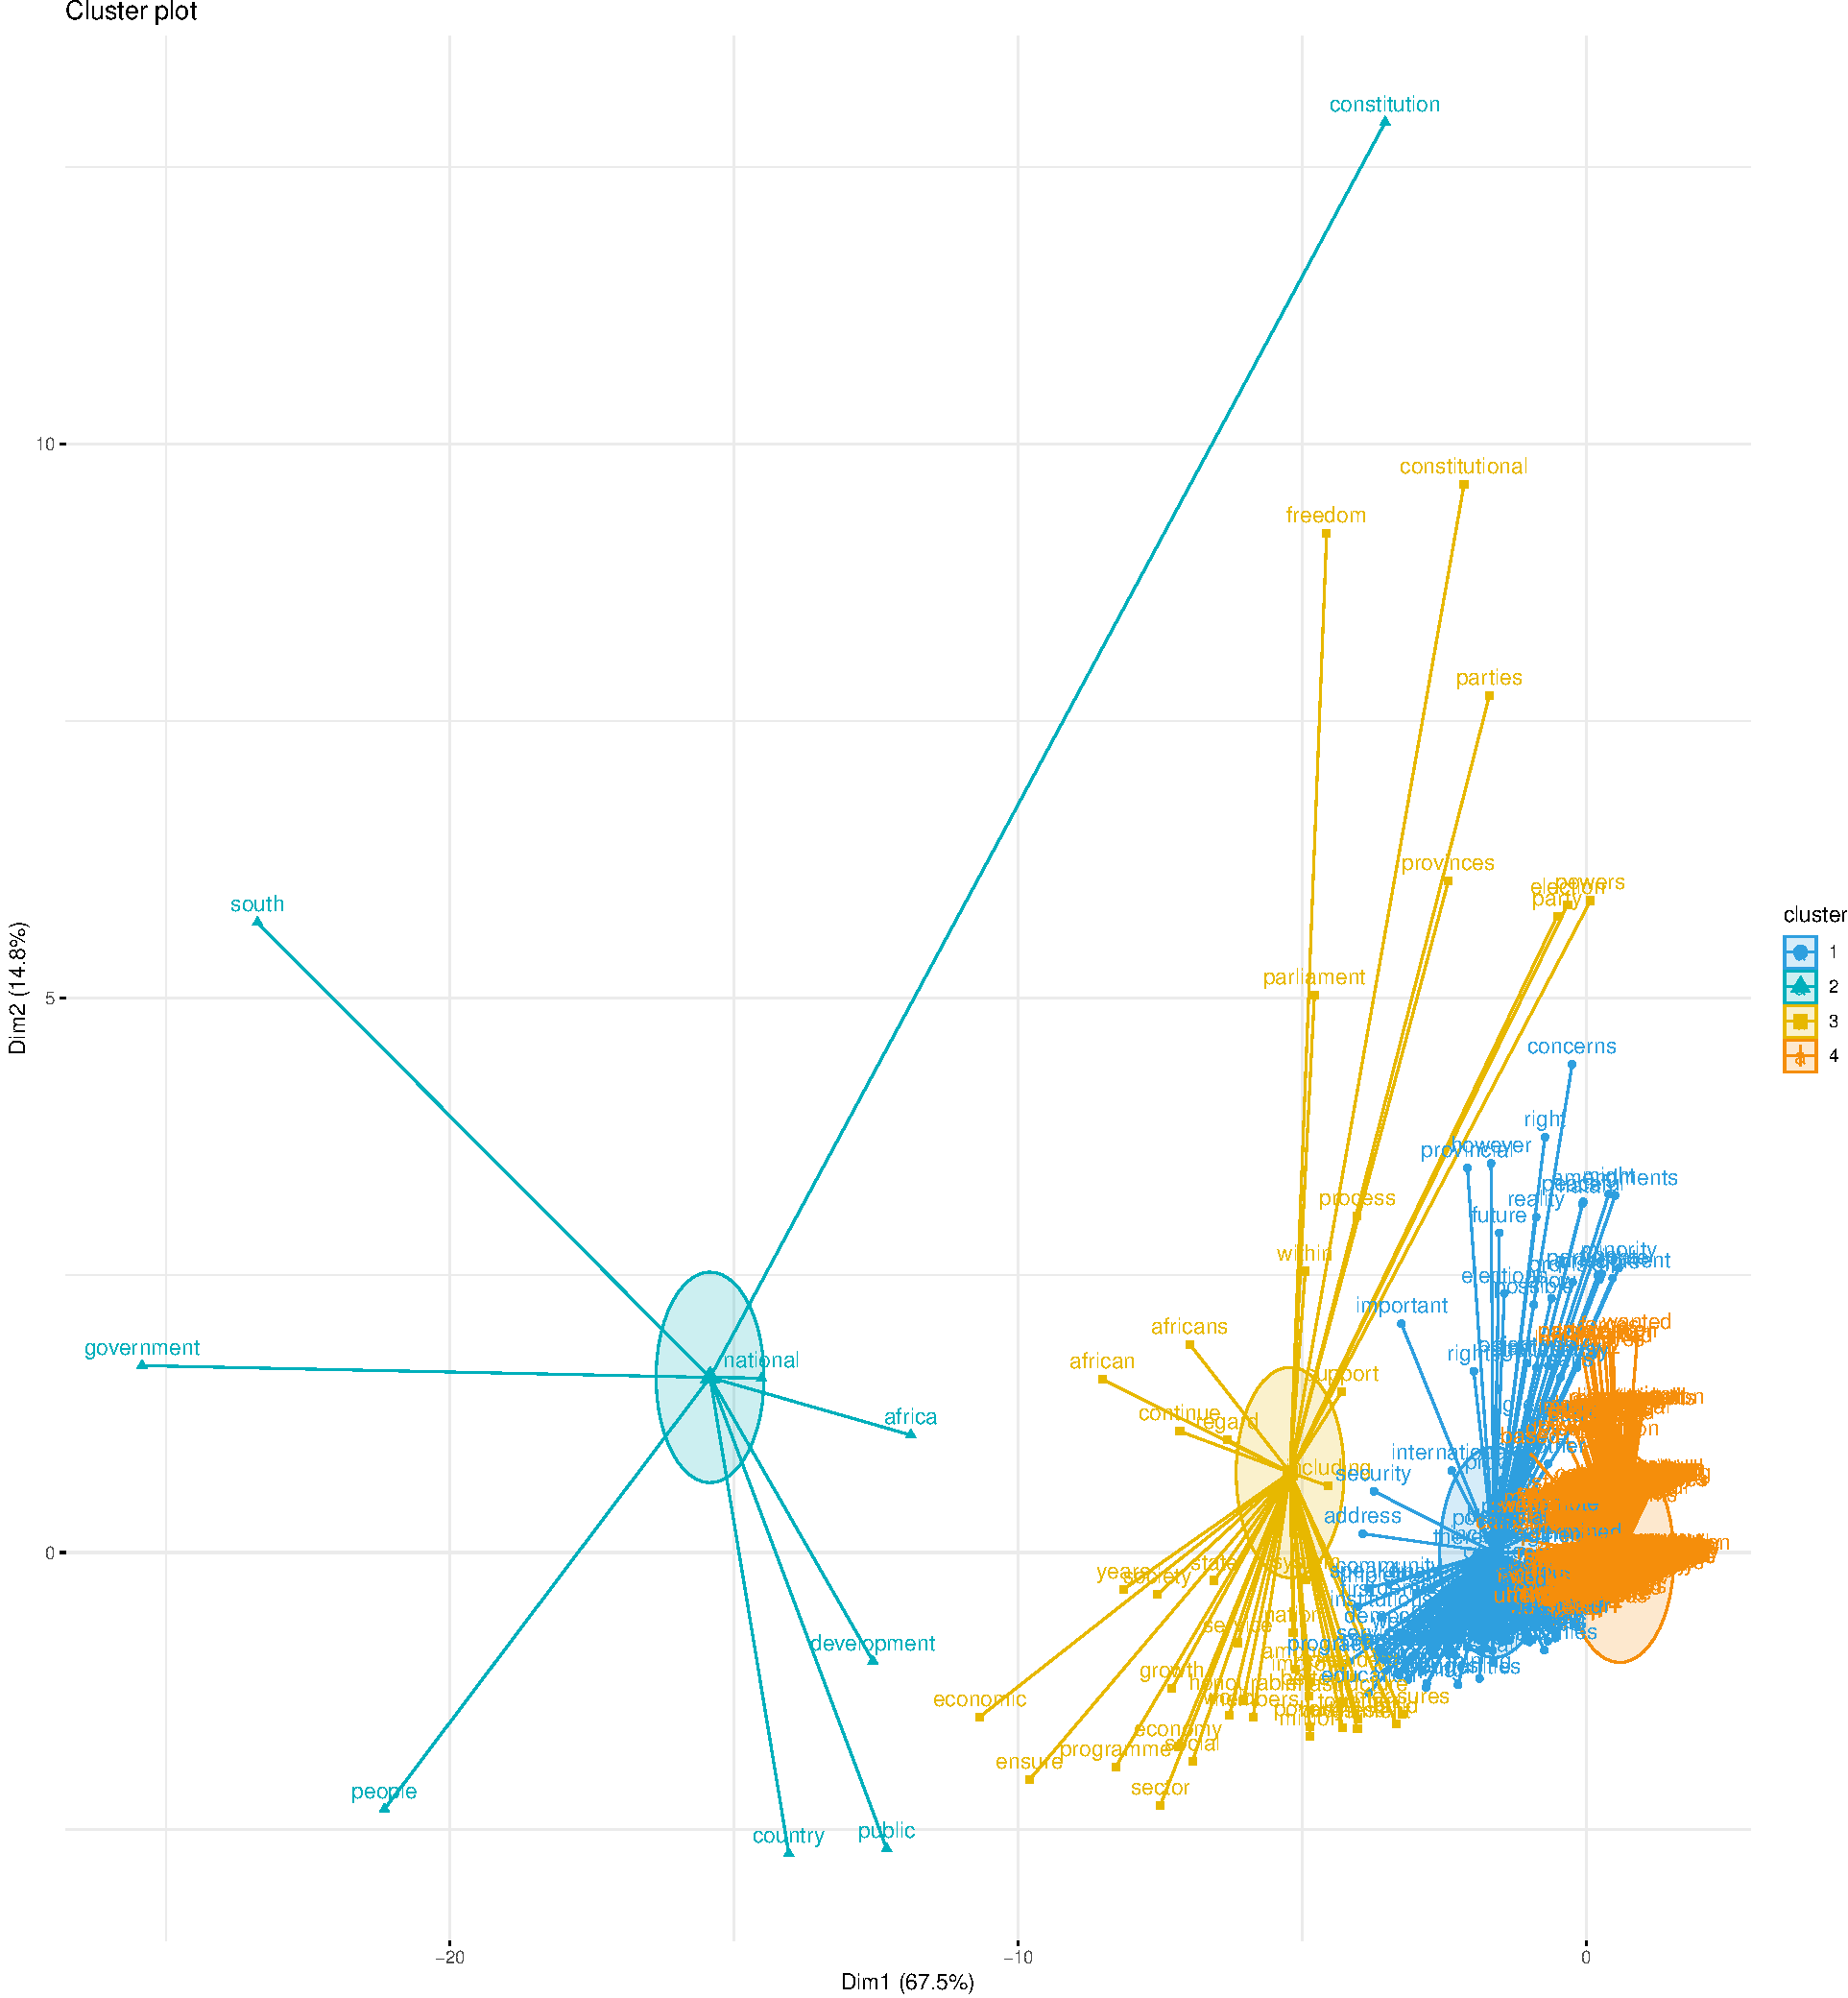
\includegraphics{datasci_fi_Assignment_2_files/figure-latex/kmeans -1} 

}

\caption{K means clustering of speech words of the 5 presidents}\label{fig:kmeans }
\end{figure}

From the illustration above the following remarks can be made :

\begin{itemize}

\item


\end{itemize}

\subsection{Sentiment Analysis}

The SONA of before and after the elections over the years are compared
to determine whether there is an inherent tone difference.The
\emph{bing} lexicon was utilized in this analysis.The sentiment of the
words in the lexicon were summed up to determine the net sentiment which
will be referred to as polarity.Below are the results

\begin{figure}[H]

{\centering 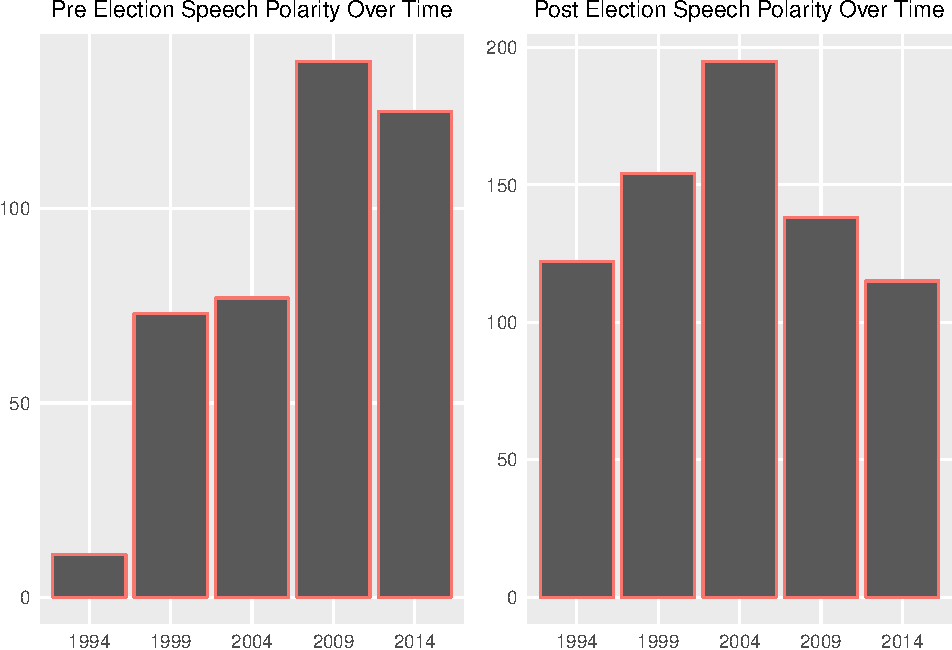
\includegraphics{datasci_fi_Assignment_2_files/figure-latex/pre_post_sentiment -1} 

}

\caption{Pre vs Post Election Speech Sentiment over time}\label{fig:pre_post_sentiment }
\end{figure}

From the illustration above the following remarks can be made :

\begin{itemize}

\item There is an interesting behavior in the first 3 election years (1994,1999,2004) there was an improvement in overall sentiment after the elections,however in the more recent 2 election years (2009,2014) there has been a more cautionary tone after elections  
\item The biggest  overall sentiment disparities before and after elections occur in 2004 and 2009.The 2004 pre/post comparison is interesting - both speeches were done by Mbeki and it showed the highest increase in net sentiment in any given year.This could be due to the fact that Mbeki had just won his second election and wanted to reassure the country with a positive speech.The 2009 pre/post comparison is counter intuitive-  one would expect that given that when Zuma was elected into power for the first time that he would have a higher net sentiment then that of the his predecessor who was there on a temporary basis.

\end{itemize}

\begin{center}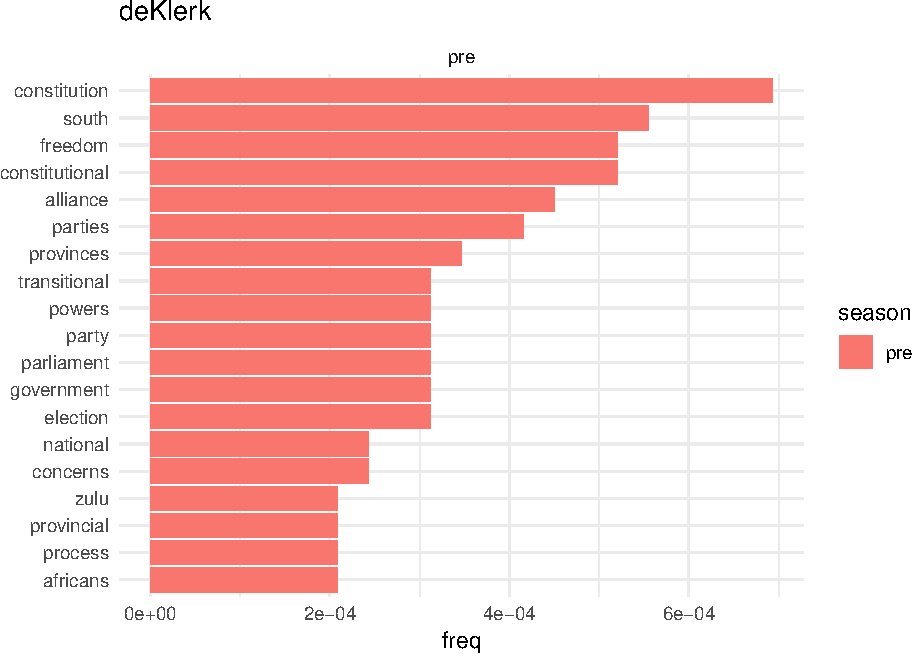
\includegraphics{datasci_fi_Assignment_2_files/figure-latex/deKlerk -1} \end{center}

\begin{center}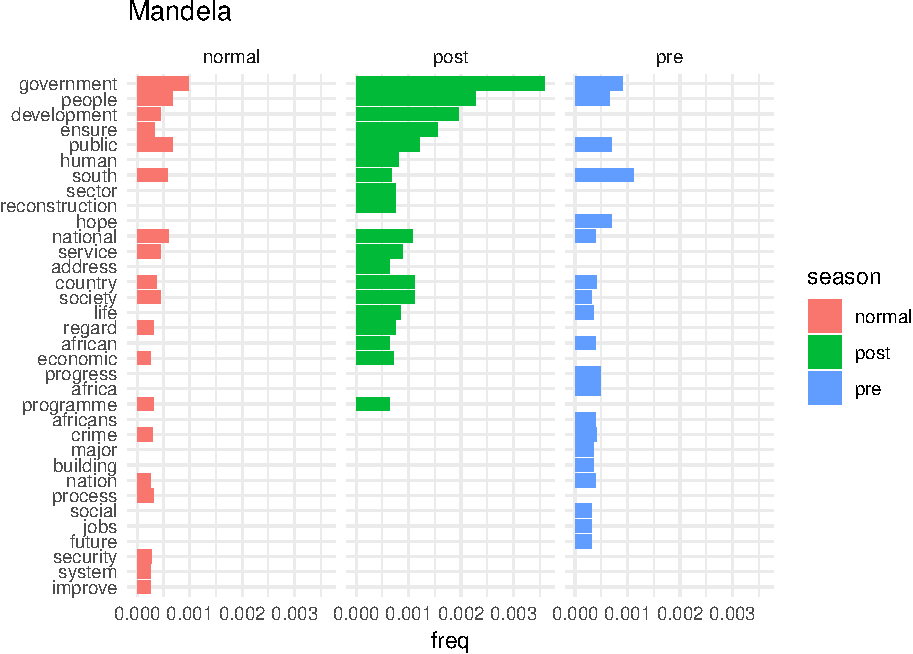
\includegraphics{datasci_fi_Assignment_2_files/figure-latex/mandela -1} \end{center}

\begin{center}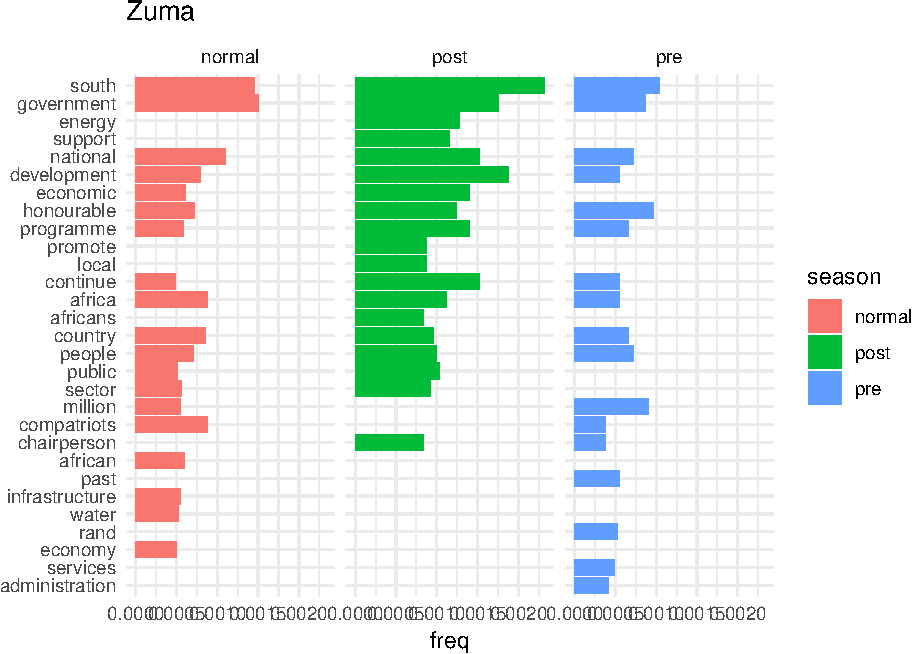
\includegraphics{datasci_fi_Assignment_2_files/figure-latex/zuma -1} \end{center}

\begin{center}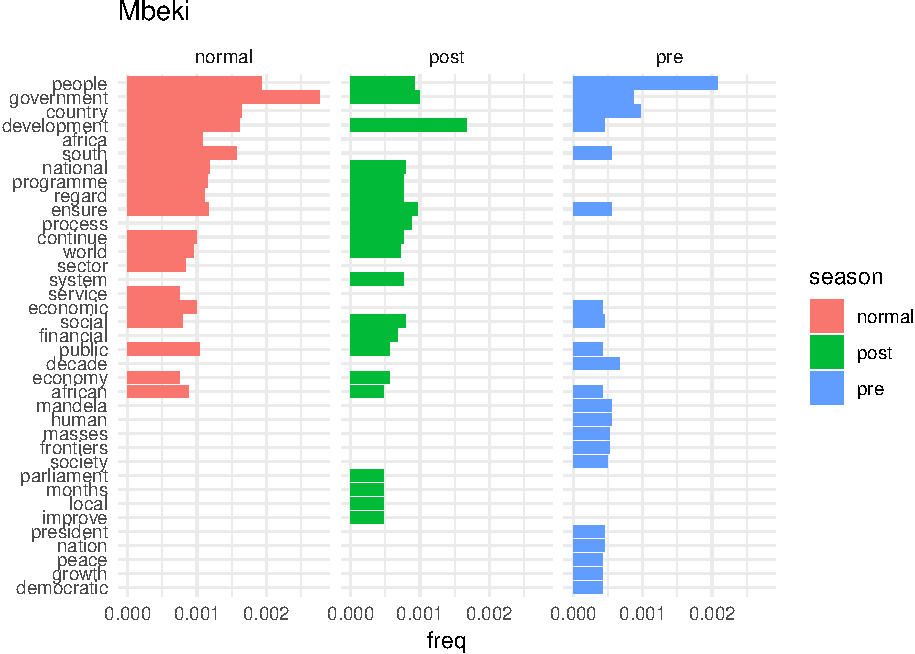
\includegraphics{datasci_fi_Assignment_2_files/figure-latex/mbeki -1} \end{center}

\begin{center}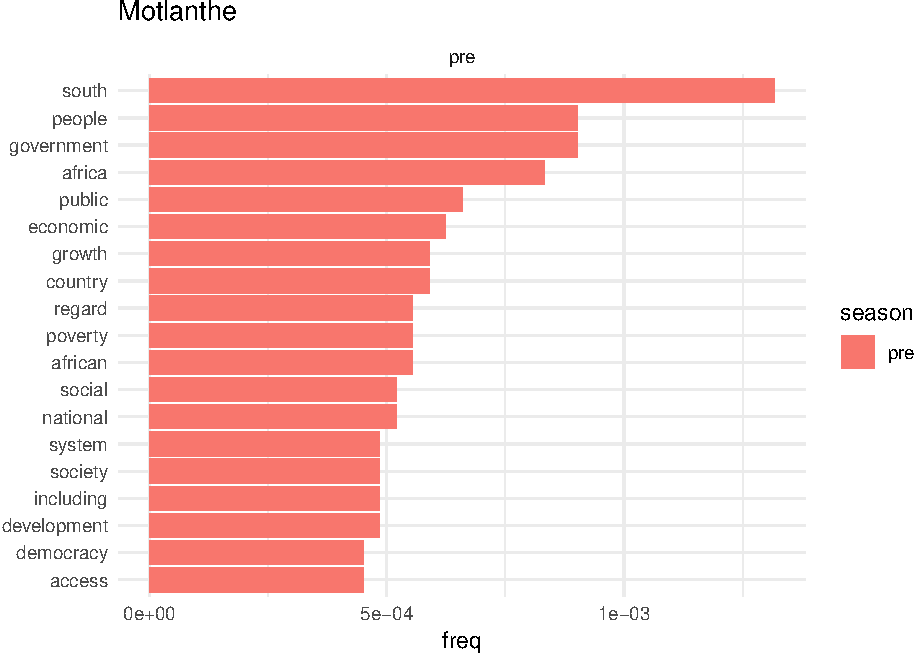
\includegraphics{datasci_fi_Assignment_2_files/figure-latex/Motlanthe -1} \end{center}

\begin{center}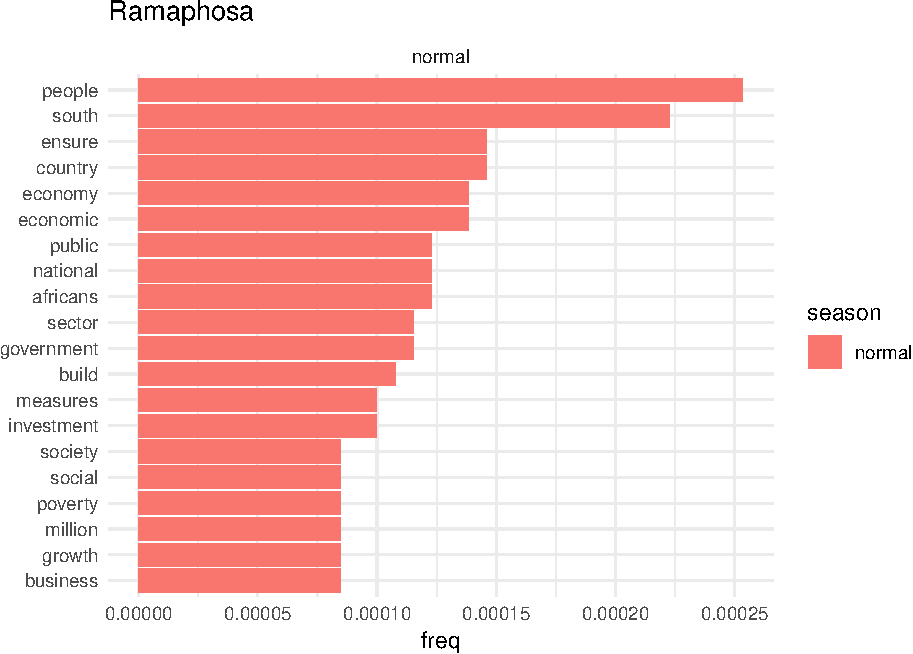
\includegraphics{datasci_fi_Assignment_2_files/figure-latex/Ramaphosa -1} \end{center}


\end{document}
